% meta.concepts: truss
% meta.tags: realistic
% acknowledge: Peter Seiler & Luke Melander graciously shared Spring 2019 course material
% source: 2019 P. Seiler AEM2011 HW 9

A Twin-Leaf Bascule bridge is a bridge where the two leafs (sections) of the bridge can rotate upwards to let
the height clearance below the bridge to increase to allow ships to pass below. Consider a parabolic Twin Leaf
Bascule bridge as shown below. Assume that in a closed position, the joint between the two leafs is a hinge
joint. The axis of the three-hinge arch ABC is a parabola with the vertex at B. Knowing that $P = 700$ kN and
$Q = 560$ kN, determine:
\begin{itemize}
  \item The components of the reaction at A.
  \item The components of the force exerted at B on segment AB.
\end{itemize}

\begin{figure}[ht!]
  \centering
  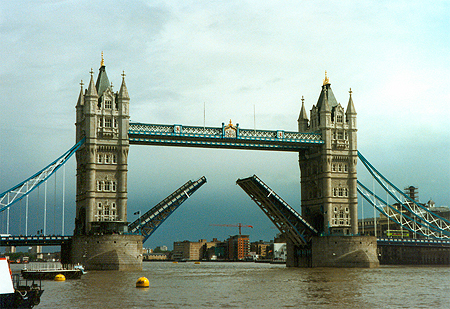
\includegraphics[width=0.4\textwidth,
	           height=0.3\textheight,
		   keepaspectratio]{figa.png}
  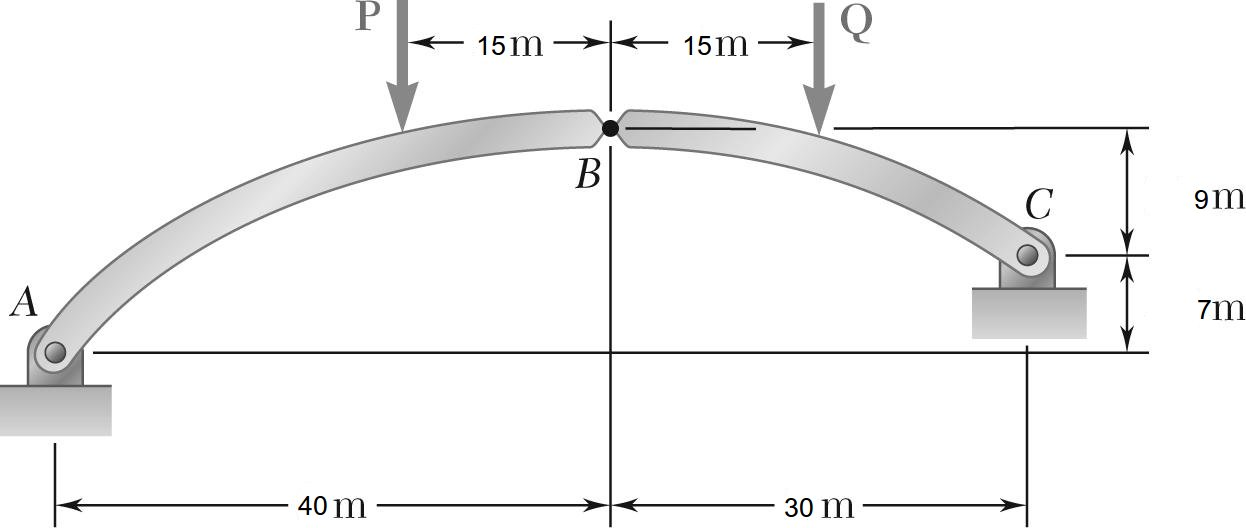
\includegraphics[width=0.4\textwidth,
	           height=0.3\textheight,
		   keepaspectratio]{figb.png}
  \caption*{Bascule Bridge (left) Simplified Diagram (right)}
\end{figure}

\iftoggle{flagSoln}{%
\vspace{.5cm}
\rule{\textwidth}{.4pt}
\vspace{.5cm}
\textbf{Solution:}
\begin{figure}[ht!]
  \centering
  \frame{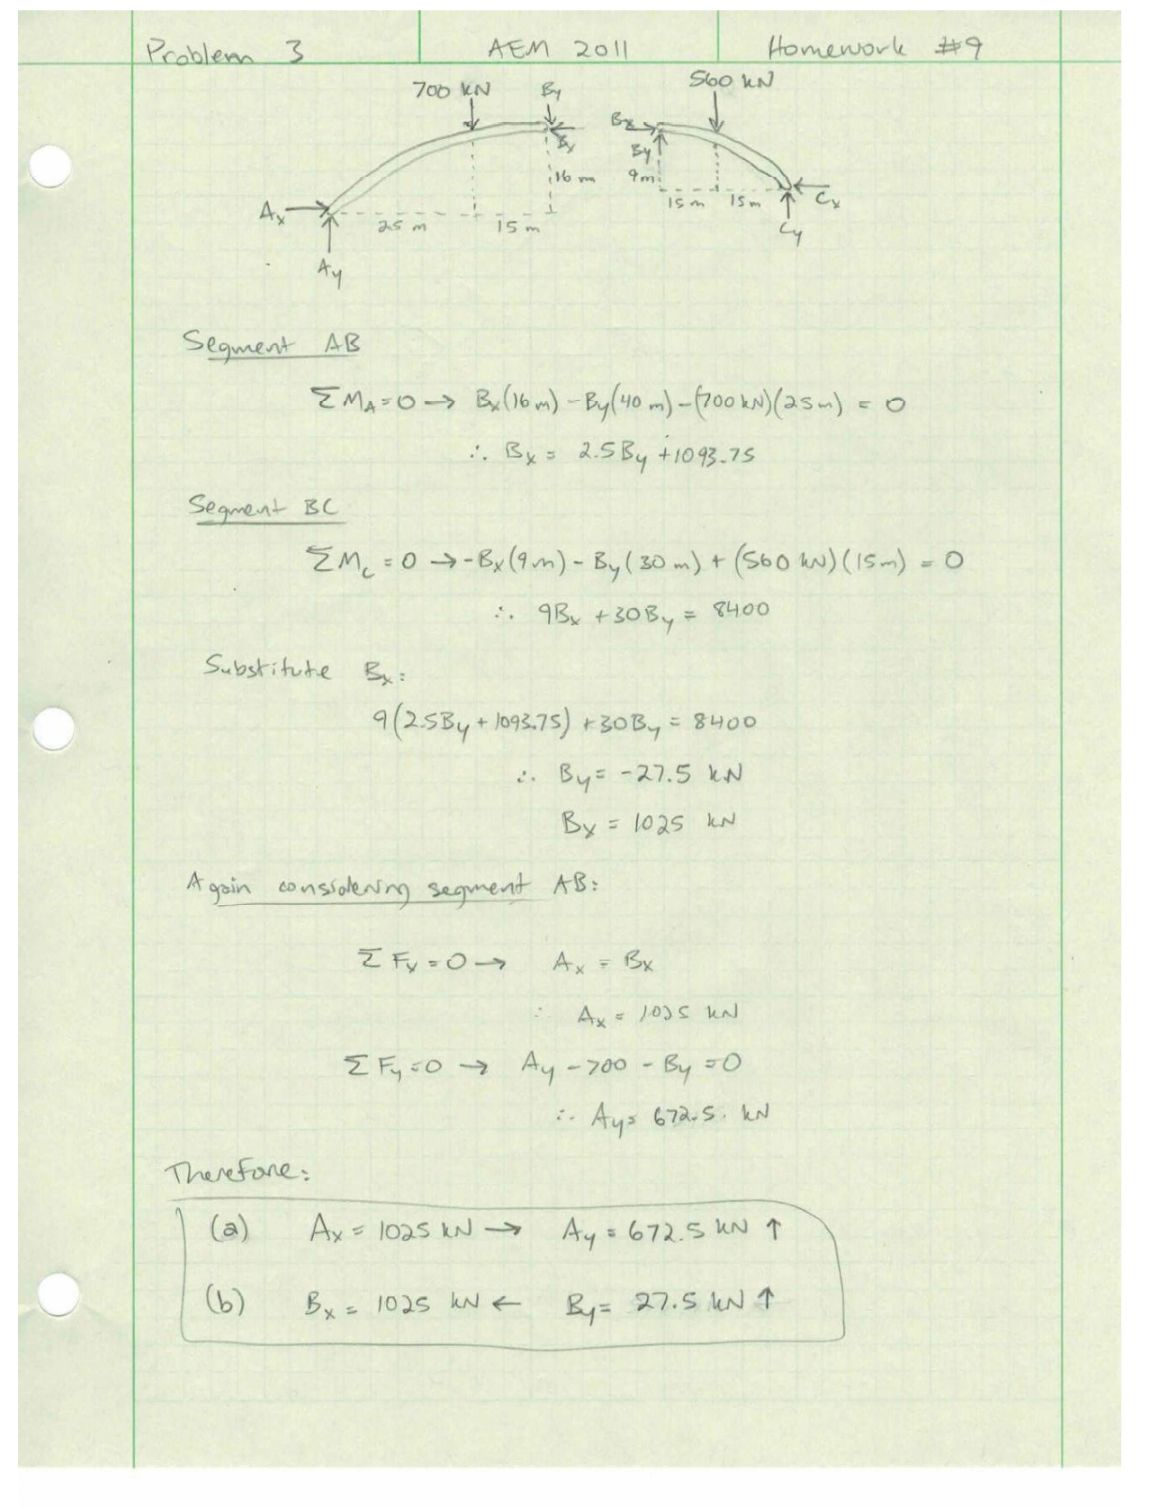
\includegraphics[width=0.9\textwidth,
	           height=0.3\textheight,
       keepaspectratio]{soln.png}}
\end{figure}
}{%
}%
